\begin{figure}[!ht]
\centering
\resizebox{\columnwidth}{!}{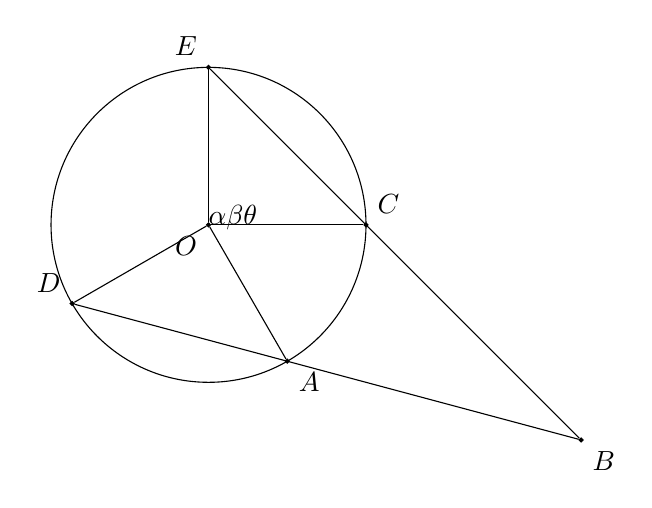
\begin{tikzpicture}
[scale=0.5,>=stealth,point/.style={draw,circle,fill = black,inner sep=0.5pt},]
%\tikzset{shift={(-3,0)}}

%innput parameters
\def\r{4}

%Labeling points
% r sin(pi/3) = 3.4641
\node (O) at (0,0)[point,label=below left:$O$] {};
\node (C) at (\r, 0 )[point,label=above right:$C$] {};
\node (A) at ({\r/2},-3.4641)[point,label=below right:$A$] {};
\node (D) at (-3.4641 , -{\r/2})[point,label=above left:$D$] {};
\node (E) at (0 , \r)[point,label=above left:$E$] {};
\node (B) at (9.4641 , -5.4641)[point,label=below right:$B$] {};


%A



%Drawing parallelogram ABCD
\draw (O) -- (A);
\draw (O) -- (C);
\draw (O) -- (E);
\draw (O) -- (D);
\draw (D) -- (B);
\draw (E) -- (B);
%\draw (C) -- (D);


\draw (O) circle (\r);
%marking angles
\tkzMarkAngle[fill=orange!50,mark=](E,O,D)
\tkzMarkAngle[fill=green!50,mark=](A,O,C)
\tkzLabelAngle[pos=0.65](E,O,D){$\alpha$}
\tkzLabelAngle[pos=0.65](A,O,C){$\beta$}
%\tkzMarkAngle[fill=orange!50,mark=](E,B,D)
\tkzLabelAngle[pos=2.65](E,B,D){$\theta$}

%
\end{tikzpicture}
}
\caption{}
\label{fig:8.5.49_circle}	
\end{figure}
%
\item {\em Construction: }See Fig. \ref{fig:8.5.49_circle}.  The input parameters are
%
\begin{align}
\label{eq:8.5.49_constr_o}
\vec{O} &= \myvec{0\\0} 
\\
\vec{C} &= \myvec{r\\0} 
\label{eq:8.5.49_constr_c}
\end{align}
Then, 
%
\begin{align}
\label{eq:8.5.49_constr_a}
\vec{A} &= r\myvec{\cos \beta \\ -\sin \beta} 
\end{align}

\subitem Equal chords subtend equal angles at the centre.  Hence 
\begin{align}
\phase{EOC} &= \phase{AOD} = \frac{360 \degree - \alpha -\beta}{2}
\\
&= 180\degree - \frac{\alpha+\beta}{2}
\end{align}
Thus, 
\begin{align}
\vec{D} &= r\myvec{\cos \brak{180^{\circ}-\frac{\alpha+\beta}{2}+\alpha} \\ \sin \brak{180^{\circ}-\frac{\alpha+\beta}{2}+\alpha}} 
\\
 &= r\myvec{-\cos \frac{\alpha-\beta}{2} \\ -\sin \frac{\alpha-\beta}{2}}
\label{eq:8.5.49_constr_d}
\\
\vec{E} &= r\myvec{\cos \brak{180^{\circ}-\frac{\alpha+\beta}{2}} \\ \sin \brak{180^{\circ}-\frac{\alpha+\beta}{2}}}
\\
 &= r\myvec{-\cos \frac{\alpha+\beta}{2} \\ \sin \frac{\alpha+\beta}{2}}
\label{eq:8.5.49_constr_e}
\end{align}
\subitem $\vec{B}$ can be found as the intersection of $AD$ and $CE$.
